\part{Gaussian Graphical Models}

A graphical model is a probabilistic models associating relations between random variables to a graph. The random variables of the model are represented by nodes in the graph and conditional independence relations are represented by missing edges between the corresponding nodes of the graph.

Consider a random vector $X$ distributed according to the \textit{multivariate Gaussian} distribution $N_p(0, \Omega^{-1})$ where $\Omega \in \S^p_{\succ 0}$ is the inverse of the \textit{covariance matrix} $\Sigma$ and is called the \textit{precision matrix}. The density of $X$ is then
\begin{equation} \label{eq-density-gaussian}
    f(x; \Omega) = (2\pi)^{-p/2} |\Omega|^{1/2} \expfc{-\frac{1}{2} \trB{xx^\top \Omega} }.
\end{equation}
We clearly see that the multivariate Gaussian distribution is an exponential family with canonical parameter $\Omega$ and sufficient statistic $\frac{1}{2}xx^\top$. 

We now introduce some notation that will be convenient when working with covariance and precision matrices of a random variable $X \sim N_p(0, \Omega^{-1})$. First, since most matrices manipulated will be referencing quantities related to entries of $X$, indexing of matrices and derived matrices will be done with respect to the entry of $X$ instead of row or column number of a matrix. For instance if $A, B \subset [p]$, then $\Sigma_{A, B}$ is the $|A|$ by $|B|$ matrix with
\begin{equation*}
    (\Sigma_{A, B})_{ab} = \cov[X_a, X_b] \ \ \textrm{for all } a \in A, b \in B.
\end{equation*}
\
We choose to parametrize the multivariate Normal distribution in terms of the precision matrix because of its special role in the context of graphical models. Indeed, the conditional independence relations of the entries a random vector $X \sim N_p(0, \Omega)$ are characterized by the sparsity patterns of the precision matrix $\Omega$.
\
\begin{lemma}
    Let $X \sim N_p(\mu, \Sigma)$ and let $i, j \in [p]$, then
    \begin{equation*}
        \Omega_{ij} = 0 \iff X_i \independent X_j | X_{[p] \setminus \eset{i,j}}.
    \end{equation*}
\end{lemma}
\begin{proof}
    By Lemma \ref{lem-gaussian-cond}, we have that the bivariate vector $X_{\eset{i,j}}$ is Gaussian with covariance matrix $\Sigma_{\eset{i,j}|[p]\setminus\eset{i,j}}$ equal to the Schur complement of $\Sigma_{[p] \setminus \eset{i,j}}$. The claim of this lemma is thus equivalent to 
    \begin{equation*}
        \Omega_{ij} = 0 \iff \Sigma_{\eset{i,j}|[p]\setminus\eset{i,j}}\ \textrm{is diagonal}.
    \end{equation*}
    Using the Schur complement inverse property, we have 
    \begin{equation*}
        \Sigma_{\eset{i,j}|[p]\setminus\eset{i,j}} 
        = \left[\Omega_{\eset{i,j}}\right]^{-1} 
        = \begin{pmatrix}
            \Omega_{ii} & \Omega_{ij}\\
            \Omega_{ji} & \Omega_{jj}
            \end{pmatrix}^{-1}
        = \frac{1}{|\Omega_{\eset{i,j}}|} \begin{pmatrix}
            \Omega_{jj} & -\Omega_{ij}\\
            -\Omega_{ji} & \Omega_{ii} 
            \end{pmatrix}^{-1}.
    \end{equation*}
    Hence, $\Sigma_{\eset{i,j}|[p]\setminus\eset{i,j}}$ is diagonal if and only if $\Omega_{ij} = 0$.
\end{proof}

Consider a graph $\G = (\Gamma, E)$ with nodes $\Gamma = \{1, \ldots, p\}$. We say that $X$ satisfies the \textit{Gaussian graphical model} with graph $\G$ if $X \sim N_p(0, \Omega)$ and
\begin{equation} \label{eq-ggm}
    \Omega_{i j} = 0 \iff \eset{i,j} \notin E.
\end{equation}
This property corresponds to the pairwise Markov property in graphical model theory. All together, we find that the independence relations of the entries of $X$, the connectivity of the nodes in $\G$ and the sparsity pattern of $\Omega$ are all the same concept viewed from a different angle which each on its own will help in studying them.

We now study properties of the maximum likelihood estimator in a Gaussian graphical model, largely following the presentation of Uhler \cite[Section 9]{maathuis2018handbook}.

Consider now a sample $X = (X^{1}, \ldots, X^{n})$ from a Gaussian distribution. The log-likelihood function for a precision matrix $\Omega \in \S^p_{\succ 0}$ obtained from (\ref{eq-density-gaussian}) is
\begin{equation*}
    \ell(\Omega; X) = \frac{n}{2} \log |\Omega| - \frac{1}{2}\tr[XX^\top\Omega].
\end{equation*}
Rewriting it in terms of the sufficient statistic $S = n^{-1}XX^\top$, we have
\begin{equation} \label{eq-likelihood}
    \ell(\Omega; S) = \frac{n}{2}\log |\Omega| - \frac{n}{2}\tr[S\Omega].
\end{equation}
In the \textit{saturated model} where no constraints are put on the entries of $\Omega$, the maximum likelihood estimator is defined when $S \in S^p_{\succ 0}$ and is equal to
\begin{equation*}
    \hat\Omega = S^{-1}.
\end{equation*}
However, if we are interested in estimating the maximum likelihood estimator $\hat\Omega$ of a Gaussian graphical model with graph $\G = ([p], E)$, the solution $\hat\Omega$ must lie in the subset $\S(\G)$ of $\S^p_{\succ 0}$ in which the conditional independence relations encoded in $\G$ are satisfied. This subset is directly given by Equation (\ref{eq-ggm}), $\S(\G) = \{ \Omega \in \S^p_{\succ 0} : \Omega_{ij} = 0 \textrm{ if } i \neq j \textrm{ and } \eset{i,j} \notin E \}$. We are then left with the following optimization problem
\begin{align} \label{eq-primal}
    \begin{split}
        &\underset{\Omega \in \S^p_{\succ 0}}{\textrm{maximize}}\ \  \log |\Omega| - \tr[S\Omega]\\
        &\textrm{subject to}\ \ \Omega \in \S(\G).
    \end{split}
\end{align}
Since the Gaussian graphical model condition is a linear constraint, the set $\S(\G)$ is the is a convex cone. Showing that the objective function in (\ref{eq-primal}) is concave would imply that maximum likelihood estimation in Gaussian graphical models is a convex optimization problem which would allow us to bring new insights to the problem by studying its dual formulation. We start by proving that the objective function is indeed concave.
\begin{lemma}
    The function $f : \S^p_{\succ 0} \rightarrow \R, X \mapsto \log |X| - \trB{SX}$ is concave.
\end{lemma}
\begin{proof}
    Since the sum of a linear function and a concave function is concave, and $\trB{SX}$ is linear in $X$, it is sufficient to show that the logarithm of the determinant of a matrix is a concave function. To do this, let us consider the line $\eset{ U + tV : t \in \R }$ for $U, V \in \S^p_{\succ 0}$. We can show that $X \mapsto \log |X|$ is concave on $\S^p_{\succ 0}$ by showing that $g(t) = \log |U + tV|$ is concave. Since $U \in \S^p_{\succ 0}$, both $U^{1/2}$ and $U^{-1/2}$ exist and we have 
    \begin{align*}
        g(t)
        &= \log |U + tV| \\
        &= \log |U^{1/2}(1_p + tU^{-1/2}VU^{-1/2}|\\
        &= \log |U| + \log |1_p + tU^{-1/2}VU^{-1/2}|\\
        &= \log |U| + \sum_{i=1}^p \log (1 + t\lambda_i),
    \end{align*}
    where $\lambda_i$ are the eigenvalues of $U^{-1/2}VU^{-1/2}$ and we use that the eigenvalues of $1_p + tU^{-1/2}VU^{-1/2}$ are $1 + t\lambda_i$. Since each $\log (1 + t\lambda_i)$ is concave in $t$, we have that $g$ is concave, completing the proof.
\end{proof}

We can now study the dual problem to (\ref{eq-primal}). The Lagragian of the maximum likelihood estimation in Gaussian graphical models is
\begin{align*}
    \mathcal{L}(\Omega, \nu)
    &= \log |\Omega| - \tr[S\Omega] - 2 \sum_{\eset{i, j} \notin E} \nu_{ij}\Omega_{ij}\\
    &= \log |\Omega| - \sum_{i=1}^p S_{ii}\Omega_{ii} - 2 \sum_{\eset{i,j} \in E} S_{ij}\Omega_{ij} - 2 \sum_{\eset{i, j} \notin E} \nu_{ij}\Omega_{ij}
\end{align*}
The Lagrange dual $H$ of (\ref{eq-primal}) is given by $H(\nu) = \mathcal{L}(\Omega^\nu, \nu)$ where $\Omega^\nu$ is the maximizer of $\mathcal{L}(\Omega, \nu)$. Derivating the expression of $\mathcal{L}(\Omega, \nu)$, we get that the inverse $\Sigma^\nu$ of $\Omega^\nu$ satisfies
\begin{equation*}
    \Sigma^\nu_{ij} = \begin{cases}
        S_{ij}\ \textrm{ if } i = j \textrm{ or } \eset{i, j} \in E\\
        \nu_{ij}\ \textrm{otherwise}.
    \end{cases}
\end{equation*}
Note that $\Sigma^\nu$ is the matrix formed by replcing entries in $S$ corresponding to missing edges with entries of the dual variables $\nu_{ij}$. Replacing this in the expression for the Lagrange dual function $H$, we obain
\begin{align*}
    H(\nu) 
    &= \log |\Omega^\nu| - \tr[S\Omega^\nu] - 2 \sum_{\eset{i, j} \notin E} \nu_{ij}\Omega^\nu_{ij}\\
    &= \log |\Omega^\nu| - \tr[\Sigma^\nu\Omega^\nu] + 2 \sum_{\eset{i, j} \notin E} \Sigma^\nu_{ij}\Omega^\nu_{ij} - 2 \sum_{\eset{i, j} \notin E} \nu_{ij}\Omega^\nu_{ij}\\
    &= \log |\Omega^\nu| - p = -\log |\Sigma^\nu| - p.
\end{align*}
And hence the dual to (\ref{eq-primal}) is
\begin{align} \label{eq-dual}
    \begin{split}
        &\underset{\Sigma \in \S^p_{\succ 0}}{\textrm{minimize}}\ \  -\log |\Sigma| - p\\
        &\textrm{subject to}\ \ \Sigma_{ij} = S_{ij}\ \textrm{ for all } i = j \textrm{ or } \eset{i, j} \in E
    \end{split}
\end{align}
To show that we can equivalently study problem (\ref{eq-primal}) and (\ref{eq-dual}), we must show that strong duality holds for this convex optimization problem. By \textit{Slater's constraint quantification} \cite[Section 5.3.2]{boyd2004convex}, it is enough to show that there exists an $\Omega^* \in \S^p_{\succ 0}$ that is strictly feasable for the primal problem. Since the identity matrix is positive definite and is an element of $\S(\G)$ for any $\G$, strong duality holds for any graph $\G$ and we can freely study both formulations of the optimization problem. Furthermore, problems (\ref{eq-primal}) and (\ref{eq-dual}) have a solution if and only if $\log |\Sigma| + p$ is unbounded from above in the set of feasable matrices. We have yet to study under which condition this is the case.

To that end, let us first introduce the notation $\Sigma^\G$ to represent the partial matrix found by removing entries in $\Sigma$ corresponding to missing edges in $\G$. With this notation, we can reformulate the dual problem (\ref{eq-dual}) as
\begin{align*}
        &\underset{\Sigma \in \S^p_{\succ 0}}{\textrm{minimize}}\ \  -\log |\Sigma| - p\\
        &\textrm{subject to}\ \ \Sigma^\G = S^\G.
\end{align*}
If this formulation, the dual optimization problem corresponds to a \textit{positive definite matrix completion} problem in which the matrix $\Sigma$ is partially specified from entries of the sample covariance matrix corresponding to edges present in $\G$. 

A necessary condition for a solution to the matrix completion problem to exist is that all completely specified principal submatrices $S^\G_{[p]\setminus I}$ of $S^\G$ for $I \subset [p]$ must be positive definite. The principal submatrix $S^\G_{[p]\setminus I}$ of $S^\G$ is completely specified if it contains no missing value. The necessary condition can be easily shown with the following argument: let $S^\G_{[p]\setminus I}$ be a principal completely specified submatrix of $S^\G$ such that there exists a $z \in \R^{p-|I|}\setminus \eset{0}$ with $z^\top S^\G_{-I} z \leq 0$. Then if $S^\G_+$ is the positive definite completion of $S^\G$, it holds that $x^\top S^\G_+ x \leq 0$ for $x \in \R^p \setminus \eset{0}$ with $x_I = z$ and $x_{-I} = 0$, contradicting the positive definiteness of $S^\G_+$.


However, as shown in the Example in Figure \ref{fig-no-completion}, this condition is not sufficient for the existence of a positive definite completion. Still, the following Theorem from \cite{GRONE1984109} shows that this condition is also sufficient exactly for chordal graphs.
\begin{theorem}
    For a graph $\G$, the following statements are equivalent
    \begin{itemize}
        \item[(a)] A partial matrix $M^\G$ has a positive definite completion if and only if all completely specified submatrices of $M^\G$ are positive definite.
        \item[(b)] $\G$ is chordal.
    \end{itemize}
\end{theorem}
\note{this should come before the theorem and counter example}
While proving this result is out of the scope of this thesis, it will help us bound the number of observations required for the dual maximum likelihood estimator to exist almost surely. Gross et al.\,\cite{10.3150/16-BEJ881} introduce the \textit{maximum likelihood threshold} of a graph $\G$, denoted $\t{mlt}(\G)$. The maximum likelihood treshold of a graph $\G$ is the smallest number of data points that guarantees that the maximum likelihood estimator exist almost surely in a Gaussian graphical model associated to the graph $\G$. In other words, $\t{mlt}(\G)$ is the smallest number of observations for which $S^\G$ can be completed to a positive definite matrix. For a Gaussian graphical model over $p$ variables, the rank of the sample covariance constructed from a sample of $n$ observations is $\t{rank}(S) = \min(n, p)$. Hence, if $n \geq p$, $S$ itself is a valid positive completing for $S^\G$, giving the worst case bound
\begin{equation*}
    \t{mtl}(\G) \leq p,
\end{equation*}
where equality holds if $\G$ is complete. Considering the cliques of $\G$ can be used to give a bound on $\t{mlt}{\G}$. As we have previously seen, a necessary condition for a positive definite completion of the partial matrix $S^\G$ to exist is that all completely specified principal submatrices $S^\G_{[p]\setminus I}$ of $S^\G$ for $I \subset [p]$ must be positive definite. If $\cal{C}$ is a clique of $\G$, $\cal{C}$ is complete and thus the submatrix $S^\G_C$ is a completely specified principal submatrix of $S^\G$. Since $S^\G_C$ is complete, it is positive definite with probability one if and only if $n \geq |\cal{C}|$. With $q(\G) = \max \eset{|\cal{C}| : \cal{C} \t{ is a clique of } \G}$ the maximum clique size in $\G$, we can lower bound the maximum likelihood threshold
\begin{equation*}
    q(\G) \leq \t{mlt}(\G).
\end{equation*}

\begin{figure}
    \begin{minipage}[c]{.3\linewidth}
        \centering
        \begin{gather*}
            \begin{pmatrix}
                1 & 0.9 & 0.3 & -0.9 \\
                0.9 & 1 & 0.9 & -0.7 \\
                0.3 & 0.9 & 1 & 0.9 \\
                -0.9 & -0.7 & 0.9 & 1
            \end{pmatrix}\\
            S
        \end{gather*}
    \end{minipage}
    \hfill
    \begin{minipage}[c]{.2\linewidth}
        \centering
        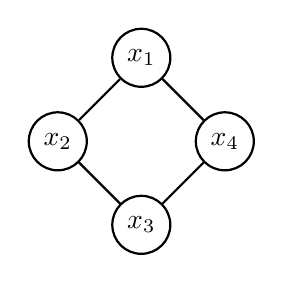
\begin{tikzpicture}[node distance={15mm}, thick, main/.style = {draw, circle}] 
            \node[main] (1) {$x_1$}; 
            \node[main] (2) [below left of=1] {$x_2$};
            \node[main] (3) [below right of=2] {$x_3$}; 
            \node[main] (4) [above right of=3] {$x_4$};
            \draw (1) -- (2);
            \draw (2) -- (3);
            \draw (4) -- (3);
            \draw (1) -- (4);
        \end{tikzpicture}
    \end{minipage}
    \hfill
    \begin{minipage}[c]{.3\linewidth} %inequalities
        \centering
        \begin{gather*}
             \begin{pmatrix}
                1 & 0.9 & ? & -0.9 \\
                0.9 & 1 & 0.9 & ? \\
                ? & 0.9 & 1 & 0.9 \\
                -0.9 & ? & 0.9 & 1
            \end{pmatrix}\\
            S^\G
        \end{gather*}
    \end{minipage}

    \caption{Example from \cite[Section 9.3]{maathuis2018handbook} of a matrix where all completely specified submatrices are positive definite but which doesn't have a positive definite completion.}
    \label{fig-no-completion}
\end{figure}





    
    



\newpage
\begin{lemma} \label{lem-gaussian-cond}
    Let $X \sim N_p(\mu, \Sigma)$ and $A, B \subset [p]$ be disjoin. Then, the conditional distribution of $X_A$ given $X_B = x_B$ is $N_|A|(\mu_{A|B}, \Sigma_{A|B})$ where
    \begin{align*}
        \mu_{A|B} = \mu_A + \Sigma_{A,B}\Sigma^{-1}_{B,B}(x_B - \mu_B) && \textrm{and} && \Sigma_{A|B} = \Sigma_{A,A} - \Sigma_{A,B}\Sigma^{-1}_{B,B}\Sigma_{B,A}.
    \end{align*} 
    One recognizes that the conditional covariance matrix $\Sigma_{A|B}$ is the Schur complement of $\Sigma_B$ in $\Sigma$.
\end{lemma}

\begin{proof}
    See \cite[Proposition C.5]{lauritzen1996}
\end{proof}
